\chapter{Entanglement}
\label{sec:4_entanglement}

In this chapter, we will finally learn about \textbf{\emph{entanglement}}: a special and unique feature of quantum mechanics.
We will begin by demonstrating how strange and counter-intuitive entanglement can be.
Then, we will move on to the definition of entangled states.
Following that, we will discuss a particular class of entangled states called ``Bell states'', which play an important role in quantum communication.
Finally, we will finish by framing entanglement as a resource for computational and communication tasks.


%%%%%%%%%%%%%%%%%%%%%
\section{CHSH Game}
\label{sec:chsh-game}
\index{CHSH game}
%%%%%%%%%%%%%%%%%%%%%

We begin with a game that will demonstrate just how wonderful and strange entangled states are.
The game is related to a proposal of four scientists named Clauser, Horn, Shimony, and Holt, though it is normally referred to as the \textbf{\emph{CHSH game}}\index{CHSH game}.
It consists of two players, labelled $A$ and $B$, and a referee denoted by $R$, as shown in Fig.~\ref{fig:chsh-game}.
The rules of the game are the following:
\begin{itemize}
    \item Referee $R$ generates two random bits, $x,y\in\{0,1\}$. Bit $x$ is sent to player $A$, and bit $y$ is sent to player $B$.
    \item Upon receiving the referee's bits, players $A$ and $B$ reply with their own bits. Player $A$ sends back a bit $a$, and player $B$ sends back bit $b$.
    \item Referee $R$ checks whether the players' bits satisfy the winning condition,
    \begin{equation}
        x\cdot y = a \oplus b,
    \end{equation}
    where $\oplus$ represents binary addition. This concludes a single round of the game.
    \item The game continues to see what percentage of the rounds the players can win.
    \item IMPORTANT: The players are not allowed to communicate once the game has started.
\end{itemize}

\begin{figure}[t]
    \centering
    \begin{tikzpicture}[->, >=stealth', auto, semithick, node distance=3cm]
    \tikzstyle{every state}=[draw=black,thick,text=black,scale=1]

    \node[state,fill=myred!50]    (R)                     {R};
    \node[state,fill=mygreen!50]   (A)[below left of=R]    {A};
    \node[state,fill=mygreen!50]   (B)[below right of=R]   {B};

    \path
    (R) edge[bend right,above,myred!60,thick]	node[yshift=1pt]{$x$}	(A)
    (R) edge[bend left,above,myred!60,thick]	node[yshift=-1pt,xshift=1pt]{$y$}	(B)
    (A) edge[bend right,left,mygreen,thick]	node[yshift=1pt]{$a$}	(R)
    (B) edge[bend left,right,mygreen,thick]	node[yshift=2pt]{$b$}	(R);

    \end{tikzpicture}
    
    \caption[CHSH game.]{CHSH game view. The players A and B attempt to collaborate to beat the referee R.}
    \label{fig:chsh-game}
\end{figure}

The players cannot communicate in order to make the game interesting, otherwise they would win every single round.
This does not mean that the players are not allowed to communicate at all.
Before the game starts, they can agree on a common strategy in order to maximize their winning chances.

Before discussing what an optimal strategy would look like, let's have a look at a few rounds of the CHSH game to become more comfortable with the rules.
\begin{table}[h]
    \setcellgapes{5pt}
    \renewcommand\theadfont{}
    \makegapedcells
    \centering
    \begin{tabular}{cccccccc}
        \hline
        & $x$ & $y$ & $a$ & $b$ & $x\cdot y$ & $a\oplus b$ \\
        \hline
        \textbf{Round 1} & 0 & 1 & 0 & 1 & 0 & 1 & \textcolor{myred}{Loss} \\
        \textbf{Round 2} & 0 & 1 & 1 & 1 & 0 & 0 & \textcolor{mygreen}{Win} \\
        \textbf{Round 3} & 1 & 1 & 1 & 0 & 1 & 1 & \textcolor{mygreen}{Win} \\
        \hline
    \end{tabular}
    \caption[CHSH game example.]{Three example rounds of the CHSH game.}
    \label{tab:4-1_chsh_rounds}
\end{table}
Table~\ref{tab:4-1_chsh_rounds} shows three example rounds of the game.
In Round 1, the referee $R$ generates the input bits with values $x=0$ and $y=1$, which are sent to the players.
The players generate their answers according to a pre-agreed strategy, and reply with $a=0$ and $b=1$.
The product of the input bits is $x\cdot y=0$, while the binary sum of the output bits is $a\oplus b=1$.
The referee determines that winning condition is not satisfied, and the players lose this round.
In Round 2, the product of input qubits is $x\cdot y=0$, and so is the binary sum of the outputs, $a\oplus b=0$. The players win this round.
Similarly for Round 3 where $x\cdot y=a\oplus b=1$.

So what is the optimal strategy that players $A$ and $B$ should follow in order to maximize their chances of winning?
We will now address this important question.
Let's begin by looking at the possible input bit pairs that the referee $R$ can generate.
There are four possible pairs, as shown in Tab.~\ref{tab:4-2_chsh_strategy}, and they are $(0,0)$, $(0,1)$, $(1,0)$, and $(1,1)$.
\begin{table}[h]
    \setcellgapes{5pt}
    \renewcommand\theadfont{}
    \makegapedcells
    \centering
    \begin{tabular}{cccccc}
        \hline
        $x$ & $y$ & $x\cdot y$ & $a=b$ & $a\oplus b$ & \\
        \hline
        0 & 0 & 0 & 0 & 0 & \textcolor{newgreen}{Win} \\
        0 & 1 & 0 & 0 & 0 & \textcolor{newgreen}{Win} \\
        1 & 0 & 0 & 0 & 0 & \textcolor{newgreen}{Win} \\
        1 & 1 & 1 & 0 & 0 & \textcolor{darkred}{Loss} \\
        \hline
    \end{tabular}
    \caption[CHSH game classical strategy.]{An example strategy for the CHSH game. Players $A$ and $B$ always reply with 0, regardless of the values of the input bits sent by the referee $R$.}
    \label{tab:4-2_chsh_strategy}
\end{table}
In the first three cases, the product of the input bits is $x\cdot y=0$. Only in the last case, when $x=y=1$, is the product equal to 1.
Realizing this, the players can agree on a strategy where they always output $a=b=0$, regardless of the value of the input bits sent by the referee.
This strategy results in the output bit binary sum $a\oplus b=0$, meaning the players win the CHSH game in three out of the four possible cases.
Since the input bits are generated uniformly at random, the probability of of a particular input pair $(x,y)$ is 1/4.
Therefore, the players have a 75\% chance of winning every round.
Not bad for such a simple strategy.

But can the players do better than that?
The answer is no, if the players are restricted to using only classical strategies.
However they can do better if they use pre-shared \textbf{\emph{entangled states}}\index{entangled state}.
A particular quantum strategy is depicted in Fig.~(\ref{fig:chsh-game_entanglement}).
Players $A$ and $B$ now share an entangled state,
\begin{equation}
    |\Phi^+\rangle = \frac{1}{\sqrt{2}} (|00\rangle + |11\rangle),
    \label{eq:4_1-phiPlus}
\end{equation}
where the first qubit corresponds to qubit $A$, while the second qubit to corresponds to qubit $B$.
\footnote{We will discuss what it means for a quantum state to be entangled in the following section.
For now, we will just accept that Eq.~(\ref{eq:4_1-phiPlus}) is entangled.
In fact, it is good to get used to this state because we will keep encountering it again and again.}
The capital Greek letter $\Phi$ is pronounced ``Phi''.
If the referee's input bit is $x=0$, player $A$ measures qubit $A$ in the $Z$ basis.
If $x=1$, player $A$ measures in the $X$ basis.
For +1 measurement outcome, player $A$ replies with $a=0$.
If the measurement outcome is -1, player $A$ replies with $a=1$.
Similar procedure applies to player $B$.
Only difference is that player $B$ measures in a \textbf{\emph{rotated basis}}\index{rotated basis}.
If the input bit is $y=0$, player $B$ measures in the $(Z+X)/\sqrt{2}$ basis.
For $y=1$, player $B$ measures in the $(Z-X)/\sqrt{2}$ basis.

% insert quantum diagram
\begin{figure}[t]
    \centering
    % \includegraphics[width=0.5\textwidth]{lesson4/CHSH_quantum_diagram.pdf}
    \begin{tikzpicture}[auto, semithick, node distance=3cm]
    \tikzstyle{every state}=[draw=black,thick,text=black,scale=1]

    \node[state,fill=red!50]    (R)                     {R};
    \node[state,fill=newgreen!50]   (A)[below left of=R]    {A};
    \node[state,fill=newgreen!50]   (B)[below right of=R]   {B};

    \path
    (R) edge[bend right,above,red!60,thick,->,>=stealth']	node[yshift=1pt]{$x$}	(A)
    (R) edge[bend left,above,red!60,thick,->,>=stealth']	node[yshift=-1pt,xshift=1pt]{$y$}	(B)
    (A) edge[bend right,left,newgreen,thick,->,>=stealth']	node[yshift=1pt]{$a$}	(R)
    (B) edge[bend left,right,newgreen,thick,->,>=stealth']	node[yshift=2pt]{$b$}	(R);

    \coordinate (qubitA) at ($(A)+(0,-1)$);
    \coordinate (qubitB) at ($(B)+(0,-1)$);

    \draw[decorate,decoration={coil,aspect=0},thick] (qubitA)  -- (qubitB);
    \filldraw[black!30,draw=black,thick] (qubitA) circle (5pt);
    \filldraw[black!30,draw=black,thick] (qubitB) circle (5pt);

    \node[] at (-3, -3.15) {qubit A};
    \node[] at (3, -3.15) {qubit B};
    \node[] at (0, -3.5) {$|\Phi^+\rangle$};

    \end{tikzpicture}
    
    \caption[Optimal quantum CHSH game strategy.]{Optimal quantum strategy for the CHSH game requires the players to pre-share an entangled state of two qubits.}
    \label{fig:chsh-game_entanglement}
\end{figure}

The above quantum strategy is a lot more complicated that the optimal classical one.
Actions of the players now depend on the inputs received from the referee.
They also need to pre-share one entangled for every round they play.
All of this extra work is well worth it however.
By following this quantum strategy, the players have probability of winning a round of 85\%.
This is an increase of 10\% compared to the optimal classical strategy.
We do not yet have the necessary tools to analyze the quantum strategy quantitatively in order to derive the winning probability.
We are about to remedy that in the remainder of this chapter.



%%%%%%%%%%%%%%%%%%%%%%%%%%%%%%%%%%%%%%%%%
\section{Entangled states}
\label{sec:4_2-entagnled_states}
%%%%%%%%%%%%%%%%%%%%%%%%%%%%%%%%%%%%%%%%%

Having seen how entangled states can be useful in the CHSH game, it is time to dicuss them in more detail.
To keep things simple, we will consider a system of two qubits.
We will use the term \textbf{\emph{local state}}\index{local state} to refer to the state of either of two qubits alone, and the term \textbf{\emph{global state}}\index{global state} to refer to the two qubits together.~\footnote{These terms can easily be extended to discuss more than one qubit in each location.}

We saw in Sec.~\ref{sec:multi-qubit} that in order to describe states of many qubits, we have to use the tensor product. For the case of the two qubits $A$ and $B$, we have the local state $\ket{\psi}_A$ of the qubit $A$, and a local state $\ket{\psi}_B$ of qubit $B$.
For concreteness, let's say that they are $\ket{0}$ and $\ket{0}$.
In order to write the global state of both qubits, we form the tensor product and we call this state $\ket{\psi}_{AB}$, which in this case is simply $\ket{00}$.
We can also consider a different state where $A$ is still in $\ket{0}$ but $B$ is now in the $\ket{+}$, a superposition of zero and one.
Again, the global state is straightforward: form the tensor product of $\ket{0}$ and $\ket{+}$,
\begin{equation}
\ket{\psi}_{AB} = \ket{0}\ket{+} = \ket{0}\left(\frac{\ket{0} + \ket{1}}{\sqrt{2}}\right) = \frac{\ket{00} + \ket{01}}{\sqrt2}.
\end{equation}

The above two examples both started with local states, which were then used to formulate the global state.
We can also ask the reverse question: given the global state, how do we write the local states of the qubits?
We can consider the global state of two qubits that we have encountered in the CHSH game in the previous section,
\begin{equation}
    \ket{\Phi^+}_{AB} = \frac{1}{\sqrt2}(\ket{00} + \ket{11})
    \label{eq:entangled_state}
\end{equation}
Identifying the local states is not that straightforward in this case.
By looking at Eq.~(\ref{eq:entangled_state}), we can see that the local state of either qubit is not quite $|0\rangle$, and it is also not quite $|1\rangle$.

At this point, it is better to get a bit more rigorous.
Let's write the local states as general pure states,
\begin{equation}
    |\psi\rangle_A = a_0|0\rangle + a_1|1\rangle, \quad |\psi\rangle_B = b_0|0\rangle + b_1|1\rangle.
\end{equation}
Taking the tensor product of $\ket{\psi}_A$ with $\ket{\psi}_B$, we arrive at the following two-qubit state, 
\begin{align}
    |\psi\rangle_{A} \otimes|\psi\rangle_{B} & = \left(a_{0}|0\rangle+a_{1}|1\rangle\right) \otimes\left(b_{0}|0\rangle+b_{1}|1\rangle\right) \nonumber\\
    & = a_0 b_0\ket{00} + a_0 b_1\ket{01} + a_1 b_0\ket{10} + a_1 b_1\ket{11}.
    \label{eq:two_qubit_separable}
\end{align}
Our goal is to find suitable probability amplitudes $a_i$ and $b_j$ such that $|\psi\rangle_{A} \otimes|\psi\rangle_{B} = |\Phi^+\rangle_{AB}$.
By comparing Eq.~(\ref{eq:entangled_state}) with Eq.~(\ref{eq:two_qubit_separable}), we see that the probablity amplitudes must satisfy two conditions,
\begin{equation}
    a_0 b_0 = a_1 b_1 = \frac{1}{\sqrt{2}}, \quad \text{ and }\quad a_0 b_1 = a_1 b_0 = 0.
\end{equation}
Let's look at the second condition first.
Either $a_0$ or $b_1$ is zero.
But setting either of them to 0, then we see that $a_0 b_0$ or $a_1 b_1$ will also be 0, meaning the first condition cannot be satisfied.
This is a remarkable discovery.
It says that \emph{not all global states can be written as a tensor product of local states}.

This leads us to the realization that there are two major classes of states.
There are \textbf{\emph{product states}}\index{product state}.
A product state is one that \textbf{\emph{can}} be written as a tensor product of local states.
Given two local states $\ket{\psi}_A$ and $\ket{\psi}_B$, we can easily find the global state by forming the tensor product.
Since we can write down the state vectors for both the global state and the local states, we say that we perfect knowledge of the local states.

The other class of quantum states are \textbf{\emph{entangled states}}\index{entangled state}.
An entangled state is a state whose global state \textbf{\emph{cannot}} be written as the tensor product of local states.
In the previous example, we have demonstrated this for an equal superposition of $\ket{00}$ and $\ket{11}$, this is in fact the case.
This is very interesting because it implies that we have perfect knowledge of the global state, but we have imperfect knowledge of local states.



%%%%%%%%%%%%%%%%%%%%%%%%%%%%%%%%%%%%%%%%%%%
\section{Bell states}
\label{sec:4_3-bell_states}
%%%%%%%%%%%%%%%%%%%%%%%%%%%%%%%%%%%%%%%%%%%

After defining what entangled states are, it is time to take a look at a very useful class of entangled states, called the \textbf{\emph{Bell states}}\index{Bell states}.
There are a total of four Bell states, 
\begin{equation}
    \begin{aligned}
        |\Phi^+\rangle & = \frac{1}{\sqrt{2}} \left( |00\rangle + |11\rangle \right), & 
        |\Phi^-\rangle = \frac{1}{\sqrt2} \left( |00\rangle - |11\rangle \right), \\
        |\Psi^+\rangle & = \frac{1}{\sqrt{2}} \left( |01\rangle + |10\rangle \right), & 
        |\Psi^-\rangle = \frac{1}{\sqrt2} \left(|01\rangle - |10\rangle \right).
    \end{aligned}
\end{equation}
We have already encountered the equal superposition of $|\Phi^+\rangle$.
Its counterpart is the $\ket{\Phi^-}$ (``phi minus'') state, where the $\ket{00}$ and $\ket{11}$ have opposite phase, as shown represented by the minus sign.
There are two more states, $\ket{\Psi^+}$ (``psi plus'') and $\ket{\Psi^-}$ (``psi minus''), which are superpositions of \ket{01} and \ket{10}, with \ket{\Psi^-} having opposite phase between the two terms. 
We will encounter these states countless number of times in the context of quantum communication.~\footnote{In some texts and papers, more commonly but not exclusively older ones, you will see these states written using the lower-case Greek letters $\phi$ (phi) and $\psi$ (psi).  In this book, we will use the capital Greek letters when referring to the Bell pairs and the lower-case letters when referring to specific variables.} 

The Bell states form an orthogonal basis for the space of two qubits.
This means that any state vector of two qubits can be written in terms of the four Bell states.
We begin with rewriting the computational basis states of two qubits $\{\ket{00},\ket{01},\ket{10},\ket{11}\}$ in terms of the Bell states.
It is not too difficult to verify that the following equalities are indeed true,
\begin{equation}
    \begin{aligned}
    |00\rangle &=\frac{1}{\sqrt{2}}\left(\left|\Phi^{+}\right\rangle+\left|\Phi^{-}\right\rangle\right), & 
    \ket{01} = \frac{1}{\sqrt2}(\ket{\Psi^{+}} + \ket{\Psi^{-}}), \\
    |10\rangle &=\frac{1}{\sqrt{2}}\left(\left|\Psi^{+}\right\rangle-\left|\Psi^{-}\right\rangle\right), & 
    \ket{11} = \frac{1}{\sqrt2}(\ket{\Phi^{+}} - \ket{\Phi^{-}}).
    \label{eq:comp_to_bell_basis}
    \end{aligned}
\end{equation}
An arbitrary two-qubit pure state can be written in the computational basis as follows,
\begin{equation}
    |\psi\rangle=\alpha|00\rangle+\beta|01\rangle+\gamma|10\rangle+\delta|11\rangle,
\end{equation}
where the probability amplitude satisfy the usual normalization condition, $|\alpha|^2+|\beta|^2+|\gamma|^2+|\delta|^2=1$.
Using Eq.~(\ref{eq:comp_to_bell_basis}), this pure state can be readily written in the Bell basis,
\begin{equation}
    |\psi\rangle=\frac{\alpha+\delta}{\sqrt{2}}\left|\Phi^{+}\right\rangle+\frac{\alpha-\delta}{\sqrt{2}}\left|\Phi^{-}\right\rangle+\frac{\beta+\gamma}{\sqrt{2}}\left|\Psi^{+}\right\rangle+\frac{\beta-\gamma}{\sqrt{2}}\left|\Psi^{-}\right\rangle.
    \label{eq:psi_bell_basis}
\end{equation}
Note that since we have changed the basis the probability amplitudes have transformed accordingly.

We have so far been dealing with single-qubit measurements.
Such measurements only had two possible outcomes.
Measuring in the Pauli $Z$ basis would project the initial state onto either $\ket{0}$ or $\ket{1}$.
If the basis of measurement is the Pauli $X$, then the post-measurement state will be either $\ket{+}$ or $\ket{-}$.
However, there is no reason to stop at single-qubit measurements.
We can extend our previous discussion to two-qubit measurements.
Not only that, we can consider two-qubit measurement in an entangled basis.
An example of this is \textbf{\emph{measurement in the Bell basis}}\index{Bell-basis measurement}.
Measuring a general two-qubit state $\ket{\psi}$ in the Bell basis has now four possible outcomes.
The post-measurement state can be any of the four Bell states $\{\ket{\Phi^+}, \ket{\Phi^-}, \ket{\Psi^+}, \ket{\Psi^-}\}$.
Using Eq.~(\ref{eq:psi_bell_basis}), we can easily determine the probabilities of these outcomes,
\begin{equation}
    \begin{aligned}
    &\operatorname{Prob}\left\{|\Phi^{+}\rangle\right\}=\frac{|\alpha+\delta|^{2}}{2} \quad \operatorname{Prob}\left\{|\Phi^{-}\rangle\right\}=\frac{|\alpha-\delta|^{2}}{2} \\
    &\operatorname{Prob}\left\{|\Psi^{+}\rangle\right\}=\frac{|\beta+\gamma|^{2}}{2} \quad \operatorname{Prob}\left\{|\Psi^{-}\rangle\right\}=\frac{|\beta-\gamma|^{2}}{2}
    \end{aligned}
\end{equation}
This will be again very important because measurements in the Bell basis are crucial in many protocols in quantum communication, especially teleportation and entanglement swapping, which we will look at quite closely later in this book.

We mentioned in Sec.~\ref{sec:4_2-entagnled_states} that entangled states have the curious property that the global state is known perfectly, while it is not possible to express the state of the local qubits using pure states.
This suggests that we only have imperfect knowledge of the local states.
We will make this notion more concrete.

Consider the two-qubit state to be the $|\Phi^+\rangle$ Bell state.
Measuring this state in the Bell basis will yield the $|\Phi^+\rangle$ outcome with unit probability.
This is consistent with our interpretation of having full knowledge of the global state.
Let's see what happens if we perform a single-qubit measurement on the state $|\Phi^+\rangle$.
For example, we measure qubit $A$ in the Pauli $Z$ basis.
Since this is a single-qubit measurement, we can only two possible outcomes.
The projectors associated with these two outcomes are
\begin{equation}
    \Pi^A_{Z,+} = |0\rangle_A\langle0| \otimes I_B, \quad \text{ and } \Pi^A_{Z,-} = |1\rangle_A\langle1| \otimes I_B.
    \label{eq:local_projectors}
\end{equation}
Note the slight but necessary change of notation in Eq.~(\ref{eq:local_projectors}).
The superscript $A$ labels which local qubit is being measured, while the subscript now labels both the basis and the measurement outcome.
The probability of obtaining the +1 outcome is
\begin{align}
    \operatorname{Pr}\{+1\} & = \operatorname{Tr}\left\{\Pi^A_{Z,+} |\Phi^+\rangle_{AB}\langle\Phi^+|\right\} \\
    & = \langle\Phi^+|_{AB} \left( |0\rangle_A\langle0| \otimes I_B \right) |\Phi^+\rangle_{AB} \nonumber\\
    & = \frac{1}{2} \left( \langle00|_{AB} + \langle11|_{AB} \right) \left( |0\rangle_A\langle0| \otimes I_B \right) \left( |00\rangle_{AB} + |11\rangle_{AB} \right) \nonumber\\
    & = \frac{1}{2} \left( \langle0|0\rangle_A^2 \langle0|0\rangle_B + \langle0|0\rangle_A \langle0|1\rangle_A \langle0|1\rangle_B \right. \nonumber\\
    & + \left. \langle1|0\rangle_A \langle0|0\rangle_A \langle1|0\rangle_B + \langle1|0\rangle_A \langle0|1\rangle_A \langle1|1\rangle_B \right) \nonumber\\
    & = \frac{1}{2}. \nonumber
\end{align}
Similar calculation can be repeated for the case of the -1 measurement outcome,
\begin{equation}
    \operatorname{Pr}\{-1\} = \operatorname{Tr}\left\{\Pi^A_{Z,-} |\Phi^+\rangle_{AB}\langle\Phi^+|\right\} = \frac{1}{2}.
\end{equation}

\label{page:plus-is-pure}
At this point, you may be a little puzzled; didn't we see this same fifty-fifty behavior with a single qubit in the $\ket{+}$ state?  What is different with entanglement?  When measuring in the Z basis, it is true that we always see the fifty-fifty statistics.  However, if we measure a $\ket{+}$ in the X basis, we will always find that the state is in the $+1$ state.  We can also choose to apply a Hadamard gate to the $\ket{+}$ state and return it to a known $\ket{0}$ state.  Thus, although the qubit is in superposition, we have complete information about that superposition.  In contrast, when we hold only one qubit of an entangled pair and attempt to measure it, our results will differ.

%\rdv{This par fails to completely close the deal in demonstrating that we don't have any local information, since the outcomes are 50/50 both when we are talking about a single plus state and a Bell state.  Needs a counterpoint where we have full information?  Show that the single plus state always has a specific outcome when measuring in the X basis.} Added above.

If we change the measurement basis to a Pauli $Y$ basis, again we find that the probability of the $+1$ outcome is the same as the probability of the $-1$ outcome. It is the same for the $X$ basis, and in fact in any basis that you measure qubit $A$, you will get the same result: both outcomes are fifty-fifty. In fact, the local measurement results are uniformly random in any basis.
Remember that the global state of the system is pure.
We know exactly what it is, yet no matter in what basis we measure the states locally we are getting 50 percent one outcome and 50 percent the other outcome.
We can say that we have no knowledge of the local states of qubit $A$ and qubit $B$.
This goes back to our previous discussion about the difference between entangled states and product states. 
Since this state is entangled, the correct description of the local qubits must be given in terms of density matrices, and we can write that the state of qubit $A$ is a maximally mixed state.
The same holds for qubit $B$.
The local states of the two qubits are therefore
\begin{equation}
    \rho_A=\frac{1}{2}(|0\rangle\langle 0|+| 1\rangle\langle 1|), \quad
    \rho_B=\frac{1}{2}(|0\rangle\langle 0|+| 1\rangle\langle 1|).
\end{equation}

Just to stress how strange this is that we have a full knowledge of the global state yet we have zero knowledge of the local states, let's look at this again: qubit $A$ is a maximally mixed state. We have no knowledge about its state. The same is true for qubit $B$ considered in isolation. Yet, somehow, when we look at the state globally, we have perfect knowledge of the entire state. This distinction is addressed more in the chapter exercises.


%%%%%%%%%%%%%%%%%%%%%%%%%%%%%%%%%%%%%%%%%%%%%%%%
\section{Spontaneous parametric down-conversion}
\label{sec:4-4_spdc}
%%%%%%%%%%%%%%%%%%%%%%%%%%%%%%%%%%%%%%%%%%%%%%%%

In this section, we will learn about one possible way of producing the entangled states that we have been discussing so far.
The physical systems that will encode the qubits are photons, and the process generates entangled photon pairs is called \textbf{\emph{spontaneous parametric down-conversion}}\index{spontaneous parametric down-conversion}, or SPDC for short. There are many physical processes that can generate entangled pairs of photons, but this one is common in laboratories and will serve as our example.

The basic idea behind SPDC is illustrated in Fig.~\ref{fig:spdc}.
A high-energy \textbf{\emph{pump photon}}\index{pump photon}, pictured in green, is incident on a nonlinear crystal.
A popular choice of material for the crystal is \textbf{\emph{beta barium borate}}\index{BBO}, or BBO for short.
The pump photon interacts with atoms inside the nonlinear crystal and gets transformed into two lower-energy photons.
Often these photons are referred to as the \textbf{\emph{signal}}\index{signal photon} and the \textbf{\emph{idler}}\index{idler photon}.

\begin{figure}[t]
    \centering
    % \includegraphics[width=0.5\textwidth]{lesson4/pump.pdf}
    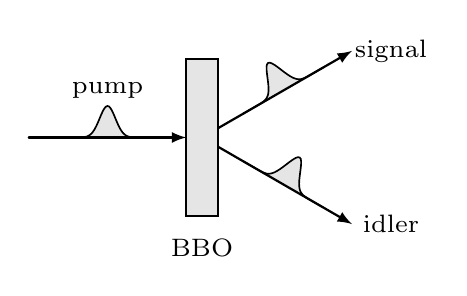
\begin{tikzpicture}[scale=2, every node/.style={scale=1.3},wave/.style={semithick,color=#1,smooth}]
        % \draw[semithick,darkred!70,decorate,decoration={coil,aspect=0,segment length=2mm}] (0.5,0.8)  -- (0.5,0.2);
        
        \begin{scope}
            \draw[wave=black, fill=black!10, variable=\x, samples at={-0.3,-0.29,...,0.3}] plot (\x-0.6, {0.2*e^(-\x*\x/0.005)+0.5});
            \draw[thick, -latex, line cap=round] (-1.1,0.5) -- (-0.1, 0.5);
            \node[black] at (-0.6,0.8) {\scriptsize pump};
        \end{scope}

        \begin{scope}[rotate around={30:(0.0,0.5)}]
            \draw[wave=black, fill=black!10, variable=\x, samples at={-0.3,-0.29,...,0.3}] plot (\x+0.6, {0.2*e^(-\x*\x/0.005)+0.5});
            \draw[thick, -latex] (0.0,0.5) -- (1.1,0.5);
        \end{scope}

        \begin{scope}[rotate around={-30:(0.0,0.5)}]
            \draw[wave=black, fill=black!10, variable=\x, samples at={-0.3,-0.29,...,0.3}] plot (\x+0.6, {0.2*e^(-\x*\x/0.005)+0.5});
            \draw[thick, -latex] (0.0,0.5) -- (1.1,0.5);
        \end{scope}
        
        \draw[thick, fill=gray!20] (-0.1,0) rectangle (0.1,1);

        % \node[text width=1.5cm] at (0.1,-0.4) {\scriptsize beta barium borate (BBO)};
        \node[] at (0,-0.2) {\scriptsize BBO};
        \node[] at (1.2,1.05) {\scriptsize signal};
        \node[] at (1.2,-0.05) {\scriptsize idler};
    \end{tikzpicture}
    \caption[Spontaneous parametric down conversion (SPDC).]{Symmetric parametric down conversion (SPDC) turns one high-energy pump photon into two lower-energy photons, with some very low probability.}
    \label{fig:spdc}
\end{figure}

``Spontaneous'' means that the process is not stimulated.
In a spontaneous process, no other input is needed, only the incoming photon of high energy that gets converted into two photons of lower energies.
(In contrast, a \emph{stimulated} process requires both the input photon and some other photon as well; a good example would be lasing.) “Parametric” means the whole process does not depend only on the intensity of the electric field but also on the phase of the field. In the context of the SPDC, it means there is a relationship between the input and output electric fields.

\begin{figure}[t]
    \centering
    \includegraphics[width=0.8\textwidth]{lesson4/4-8_spdc.pdf}
    \caption[Pump photon exciting an atom.]{A representation of the pump photon of energy $E_p$ and the energy levels of the atom. Energy level diagrams such as these are an abstraction that allows us to describe absorption and emission of photons by an atom. The circle indicates that there is a single electron in the ground state.
    The atom absorbs the energy provided by the pump photon and transitions to the excited state. The atom decays spontaneously after some time, releasing energy in the form of two photons with energies $E_s$ and $E_i$. Due to conservation of energy, we have $E_p = E_s + E_i$.}
    \label{fig:spdc-energy-levels}
\end{figure}

We can zoom into the nonlinear crystal to see what happens at the level of individual atoms interacting with single photons of the pump, as shown in Fig.~\ref{fig:spdc-energy-levels}.
We can tune the energy of the pump photons to be resonant with a particular transition frequency of the atoms inside the BBO crystal.
Therefore, to a good approximation the pump laser will only affects those two energy levels.
The lower level is called the \textbf{\emph{ground state}}\index{ground state} and the upper level is call the \textbf{\emph{excited state}}\index{excited state}.
The atom in the BBO crystal initially starts in the ground state.
The pump photon carries the right amount of energy to excite the atom.
After a short time the atom de-excites and transitions back into the ground state.

The vast majority of the time, this de-excitation is coupled with the emission of a single, high-energy photon.
With some very low probability, however, the atom emits two photons with energy $E_s$ for the signal photon and energy $E_i$ for the idler photon.
Because energy is conserved in this transition, we must have that the energy of the pump photon be equal to the sum of the energies of the outgoing photons, $E_p = E_s + E_i$.
This is the basic process of spontaneous parametric down-conversion.

Now that we have covered the basic idea of the SPDC process it is time to discuss how we can use photons encode qubits.
Qubits have two distinguishable states.
They are represented by the abstract orthogonal kets, for example $\{|0\rangle,|1\rangle\}$ or $\{|+\rangle,|-\rangle\}$.
A general state of the qubit is then written as an arbitrary superposition of these two orthogonal states.
Therefore, we require the photons to be able to possess two distinguishable \textbf{\emph{degrees of freedom}}\index{degree of freedom} which can also form superposition.
A natural choice for the photons is their \textbf{\emph{polarization}}\index{polarization}.

\begin{figure}[t]
    \centering
    \begin{tikzpicture}
        \draw[semithick,dashed,black!50] (0,0) circle (1.5cm);
        \draw[thick,latex-latex,newgreen] (-1.5,0) -- (1.5,0);
        \draw[thick,latex-latex,darkred] (0,-1.5) -- (0,1.5);
        \draw[thick,latex-latex,blue!50] (-1.06,-1.06) -- (1.06,1.06);

        \draw[-latex] (0:0.75) arc (0:45:0.75);
        \node[] at (1.0, 0.35) {\small $45\degree$};

        \node[newgreen] at (2.5,0.2) {horizontal};
        \node[newgreen] at (2.5,-0.2) {polarization};

        \node[darkred] at (0, 2.2) {vertical};
        \node[darkred] at (0, 1.8) {polarization};

        \node[blue!50] at (1.9, 1.4) {diagonal};
        \node[blue!50] at (2.15, 1.05) {polarization};
    \end{tikzpicture}
    \caption[Linear polarization of light.]{Linear polarization of light. Horizontally polarized light can be superposed with vertically polarized one to form diagonal polarization.}
    \label{fig:polarization}
\end{figure}

Natural light is composed of many electromagnetic waves, each oscillating in a different direction.
It is this direction of oscillations that we call polarization\footnote{We will not cover polarization in depth as this would require delving into electromagnetism. We will address electromagnetic theory and Maxwell's equations in great detail in our next book}.
If the electromagnetic waves are oscillating in the horizontal plane we say the light is \textbf{\emph{horizontally polarized}}\index{horizontally polarized}, as shown in Fig.~\ref{fig:polarization}.
And if the oscillations are in the vertical direction, you guessed it, the light is \textbf{\emph{vertically polarized}}\index{vertically polarized}.
These two polarizations are just two possible ones out of infinitely many.
Another example that we will prove very useful in this Section is \textbf{\emph{diagonal polarization}}\index{diagonal polarization}.
It can be viewed as a superposition of horizontally and vertically polarized light.

Distinguishing different orthogonal polarization states of light can be done easily with the help of \textbf{\emph{polarizers}}\index{polarizer}.
Polarizer is an optical element that lets through light of only certain polarization and blocks all other light.
Sunglasses are a good example of polarizing filters that are used to reduce the intensity of sunlight in order to protect our eyes.
Figure~\ref{fig:polarizer} shows what happens when light of different polarization is incident onto a polarizer.
Horizontal polarizer lets through only horizontally polarized light, while a vertical polarizer lets through only vertically polarized light.
\begin{figure}[t]
    \centering
    % \includegraphics[width=0.8\textwidth]{lesson4/linear_polarization.pdf}
    \begin{tikzpicture}[x={(0.866cm,-0.5cm)}, y={(0.866cm,0.5cm)}, z={(0cm,1cm)}, scale=0.8, >=stealth, axis/.style={thick,->}, wave/.style={thick,color=#1,smooth}, polaroid/.style={fill=black!30!white, opacity=0.7}]

    \begin{scope}
    \coordinate (O) at (0,0,0);

    \draw[thick] (-3.25,0,0) -- (O);

    % Electric fields
    \draw[wave=newgreen, fill=newgreen!60, fill opacity=0.2, variable=\x,samples at={-3.14,-3.13,...,0}] plot (\x,{sin(2*\x r)},0);

    \draw[wave=lightred, fill=lightred!60, fill opacity=0.2, variable=\x,samples at={-3.14,-3.13,...,0}]
        plot (\x,0,{sin(2*\x r)});

    % Polarizer
    \filldraw[polaroid] (0,-2,-1.5) -- (0,-2,1.5) -- (0,2,1.5) -- (0,2,-1.5) -- (0,-2,-1.5) node[below, sloped, near end]{polarizer};
    \draw[thick,latex-latex] (0,-1.75,-1) -- (0,-0.75,-1);

    \draw[wave=newgreen, fill=newgreen!60, fill opacity=0.2, variable=\x,samples at={0,0.01,...,3.14}] plot (\x,{sin(2*\x r)},0);

    \draw[axis] (O) -- (4,0,0) node [right] {};
    \draw[axis] (O) -- (0,2.5,0) node [right,newgreen] {$H$};
    \draw[axis] (O) -- (0,0,2) node [above,lightred] {$V$};
    \end{scope}

    \begin{scope}[xshift=7cm]
    % Axis
    \coordinate (O) at (0,0,0);
    \draw[axis] (O) -- (4,0,0) node [right] {};
    \draw[axis] (O) -- (0,2.5,0) node [right,newgreen] {$H$};
    \draw[axis] (O) -- (0,0,2) node [above,lightred] {$V$};

    \draw[thick] (-3.25,0,0) -- (O);

    % Electric fields
    \draw[wave=newgreen, fill=newgreen!60, fill opacity=0.2, variable=\x,samples at={-3.14,-3.13,...,0}] plot (\x,{sin(2*\x r)},0);

    \draw[wave=lightred, fill=lightred!60, fill opacity=0.2, variable=\x,samples at={-3.14,-3.13,...,0}]
        plot (\x,0,{sin(2*\x r)});

    % Polarizer
    \filldraw[polaroid] (0,-2,-1.5) -- (0,-2,1.5) -- (0,2,1.5) -- (0,2,-1.5) -- (0,-2,-1.5) node[below, sloped, near end]{polarizer};
    \draw[thick, <->] (0, -1.5,-1) -- (0, -1.5, 0);

    \draw[axis] (O) -- (0,2.5,0) node [right,newgreen] {$H$};
    \draw[axis] (O) -- (0,0,2) node [above,lightred] {$V$};

    \draw[wave=lightred, fill=lightred!60, fill opacity=0.2, variable=\x,samples at={0,0.01,...,3.14}] plot (\x,0,{sin(2*\x r)});

    \draw[axis] (O) -- (4,0,0) node [right] {};
    \end{scope}
    \end{tikzpicture}
    
    \caption[Polarizing filter.]{Horizontal polarizer only lets through light of horizontal polarization as shown in the left image. Similarly, only vertically polarized light can pass through a vertical polarizer.}
    \label{fig:polarizer}
\end{figure}

All of this discussion carries through to the level of individual photons as well.
Photons can be polarized too.
However, individual photons are quantum states and therefore we have to describe then with kets.
We label a horizontally polarized photon by the ket $|H\rangle$, and a vertically polarized photon with the ket $|V\rangle$.
Now the idea of a photon encoding a qubit becomes more clear.
We can use the horizontal polarization state $|H\rangle$ to correspond to the $|0\rangle$ state of our qubit, and the vertical polarization state $|V\rangle$ to correspond to the $|1\rangle$ state.
General pure state of the qubit $\alpha|0\rangle+\beta|1\rangle$ can be then encoded into the photon by a general superposition of the photon's polarization,
\begin{equation}
    |\psi\rangle = \alpha|H\rangle + \beta|V\rangle.
\end{equation}
For example, the equal superposition $|+\rangle$ is encoded using the diagonal polarization, that is $|D\rangle=(|H\rangle+|V\rangle)/\sqrt{2}$.
Table~\ref{tab:4-4_polarization_encoding} summarizes how the polarization degree of freedom of individual photons is used to encode a qubit.
\begin{table}[h]
    \setcellgapes{5pt}
    \renewcommand\theadfont{}
    \makegapedcells
    \centering
    \begin{tabular}{cccc}
        \hline
         & \textbf{Basis states} & \textbf{Equal superposition} & \textbf{General state} \\
        \hline
        Qubits & $\{|0\rangle,|1\rangle\}$ & $|+\rangle$ & $\alpha|0\rangle+\beta|1\rangle$ \\
        Polarized photons & $\{|H\rangle,|V\rangle\}$ & $|D\rangle$ & $\alpha|H\rangle+\beta|V\rangle$ \\
        \hline
    \end{tabular}
    \caption[Polarization encoding.]{Mapping between qubit states and their corresponding polarization-encoded photonic states.}
    \label{tab:4-4_polarization_encoding}
\end{table}

Now we are in a position to discuss how the polarization of the pump photons affects the polarization of the signal and idler photons in the SPDC.
When a pump photon of a particular polarization is incident onto a BBO crystal, it has a chance to be down-converted to a pair of photons with equal polarizations which are orthogonal to that of the pump photon\footnote{This is known as Type-I down-conversion. It is possible for the signal and idler photons to have opposite polarization to each other. This is known as Type-II down-conversion.}.
Left side of Fig.~\ref{fig:poalrization_BBO} shows a horizontally polarized pump photon being down-converted into two vertically polarized photons,
\begin{equation}
    |H\rangle_p \rightarrow |V\rangle_s|V\rangle_i.
\end{equation}
The figure also displays the \textbf{\emph{optic axis}}\index{optic axis} indicating the orientation of the BBO crystal\footnote{We do not go into much detail about the significance of the optic axis. Briefly, if light propagates parallel to the optic axis it suffers no bending or refraction. We will cover this topic in great detail in our next book.}.
Rotating the whole setup by 90\degree, as shown on the right side of Fig.~\ref{fig:poalrization_BBO}, we can down-convert a vertically polarized pump photon into a pair of horizontally polarized photons,
\begin{equation}
    |V\rangle_p \rightarrow |H\rangle_s|H\rangle_i.
\end{equation}

\begin{figure}[t]
    \centering
    % \includegraphics[width=0.5\textwidth]{lesson4/horizontal_optical_axis.pdf}
    \begin{tikzpicture}[x={(0.866cm,-0.5cm)}, y={(0.866cm,0.5cm)}, z={(0cm,1cm)}, scale=0.9, >=stealth, wave/.style={thick,color=#1,smooth}]

    \def\h{1}
    \def\w{1.2}
    \def\d{0.1}

    % 1st BBO
    \begin{scope}
    \coordinate (O) at (0,0,0);
    
    % Pump photon
    \draw[wave=newgreen, fill=newgreen!10, variable=\x, samples at={-0.35,-0.34,...,0.35}, thin] plot (\x-2,{0.5*e^(-\x*\x/0.02)},0);
    \node[newgreen] at (-2,0.89,0) {\footnotesize $|H\rangle_p$};
    \draw[newgreen,thick,line cap=round] (-3,0,0) -- (O);

    % BBO
    \draw[] (-\d,-\w,-\h) -- (-\d,-\w,\h) -- (-\d,\w,\h) -- (-\d,\w,-\h) -- cycle;
    \draw[] (-\d,\w,-\h) -- (\d,\w,-\h) -- (\d,-\w,-\h) -- (-\d,-\w,-\h) -- cycle;
    \draw[pattern=north east lines] (-\d,-\w,-\h) -- (-\d,-\w,\h) -- (\d,-\w,\h) -- (\d,-\w,-\h) -- cycle;
    \draw[pattern=north east lines] (-\d,\w,\h) -- (-\d,\w,-\h) -- (\d,\w,-\h) -- (\d,\w,\h) -- cycle;
    \draw[] (-\d,-\w,\h) -- (-\d,\w,\h) -- (\d,\w,\h) -- (\d,-\w,\h) -- cycle;
    \draw[] (\d,-\w,-\h) -- (\d,-\w,\h) -- (\d,\w,\h) -- (\d,\w,-\h) -- cycle;
    \draw[-latex,thick,line cap=round] (0,-\w,0) -- (0,{-1.5*\w},0);

    % signal photon
    \begin{scope}[rotate around z=20]
        \draw[wave=lightred, fill=lightred!10, variable=\x, samples at={-0.35,-0.34,...,0.35}, thin] plot (\x+1.7,0,{0.5*e^(-\x*\x/0.02)});
    \draw[-latex,lightred,thick,line cap=round] (O) -- (2.3,0,0);
    \end{scope}
    \node[lightred] at (1.3,1.4,0) {\footnotesize $|V\rangle_s$};

    % idler photon
    \begin{scope}[rotate around z=-20]
        \draw[wave=lightred, fill=lightred!10, variable=\x, samples at={-0.35,-0.34,...,0.35}, thin] plot (\x+1.7,0,{0.5*e^(-\x*\x/0.02)});
    \draw[-latex,lightred,thick,line cap=round] (O) -- (2.3,0,0);
    \end{scope}
    \node[lightred] at (1.6,-0.1,0) {\footnotesize $|V\rangle_i$};

    \node[] at (0.6,\w,\h/2) {\footnotesize BBO};
    \node[] at (-0.6,-\w-0.5,0) {\footnotesize optic};
    \node[] at (-0.6,-\w-0.5,-0.3) {\footnotesize axis};
    \end{scope}

    % 2nd BBO
    \begin{scope}[xshift=5.5cm]
    \coordinate (O) at (0,0,0);
    
    % Pump photon
    \draw[wave=lightred, fill=lightred!10, variable=\x, samples at={-0.35,-0.34,...,0.35}, thin] plot (\x-2,0,{0.5*e^(-\x*\x/0.02)});
    \node[lightred] at (-2.2,0.8,0) {\footnotesize $|V\rangle_p$};
    \draw[lightred,thick,line cap=round] (-3,0,0) -- (O);

    % BBO
    \draw[] (-\d,-\w,-\h) -- (-\d,-\w,\h) -- (-\d,\w,\h) -- (-\d,\w,-\h) -- cycle;
    \draw[pattern=north east lines] (-\d,\w,-\h) -- (\d,\w,-\h) -- (\d,-\w,-\h) -- (-\d,-\w,-\h) -- cycle;
    \draw[] (-\d,-\w,-\h) -- (-\d,-\w,\h) -- (\d,-\w,\h) -- (\d,-\w,-\h) -- cycle;
    \draw[] (-\d,\w,\h) -- (-\d,\w,-\h) -- (\d,\w,-\h) -- (\d,\w,\h) -- cycle;
    \draw[pattern=north east lines] (-\d,-\w,\h) -- (-\d,\w,\h) -- (\d,\w,\h) -- (\d,-\w,\h) -- cycle;
    \draw[] (\d,-\w,-\h) -- (\d,-\w,\h) -- (\d,\w,\h) -- (\d,\w,-\h) -- cycle;
    \draw[-latex,thick,line cap=round] (0,0,\h) -- (0,0,{1.5*\h});

    % signal photon
    \begin{scope}[rotate around z=20]
        \draw[wave=newgreen, fill=newgreen!10, variable=\x, samples at={-0.35,-0.34,...,0.35}, thin] plot (\x+1.7,{0.5*e^(-\x*\x/0.02)},0);
    \draw[-latex,newgreen,thick,line cap=round] (O) -- (2.3,0,0);
    \end{scope}
    \node[newgreen] at (1.3,1.4,0) {\footnotesize $|H\rangle_s$};

    % idler photon
    \begin{scope}[rotate around z=-20]
        \draw[wave=newgreen, fill=newgreen!10, variable=\x, samples at={-0.35,-0.34,...,0.35}, thin] plot (\x+1.7,{0.5*e^(-\x*\x/0.02)},0);
    \draw[-latex,newgreen,thick,line cap=round] (O) -- (2.3,0,0);
    \end{scope}
    \node[newgreen] at (2,0,0) {\footnotesize $|H\rangle_i$};

    \node[] at (0.6,\w,\h/2) {\footnotesize BBO};
    \node[] at (0.2,0.2,1.8*\h) {\footnotesize optic axis};
    \end{scope}
    \end{tikzpicture}
    \caption[Photon pair via SPDC.]{Horizontally polarized pump photons can be down-converted to a pair of vertically polarized photons by the BBO crystal as shown on the left side. Rotating the crystal by 90\degree makes it possible to convert a vertically polarized pump photon into a pair of horizontally polarized photons.}
    \label{fig:poalrization_BBO}
\end{figure}

\begin{figure}[t]
    \centering
    \begin{tikzpicture}[x={(0.866cm,-0.5cm)}, y={(0.866cm,0.5cm)}, z={(0cm,1cm)}, scale=0.9, wave/.style={thick,color=#1,smooth}]

    % 1st Case with thick BBO
    \begin{scope}
    \def\h{1}
    \def\w{1.2}
    \def\d{0.3}
    \coordinate (O) at (0,0,0);
    
    % Pump photon
    \draw[wave=blue!50, fill=blue!10, variable=\x, samples at={-0.35,-0.34,...,0.35}, thin, rotate around x=45] plot (\x-2,{0.5*e^(-\x*\x/0.02)},0);
    \node[blue!50] at (-2.1,0.89,0.2) {\footnotesize $|D\rangle_p$};
    \draw[blue!50,line cap=round,thick] (-3,0,0) -- (2*\d,0,0);

    % BBO 1
    \draw[] (-2*\d,-\w,-\h) -- (-2*\d,-\w,\h) -- (-2*\d,\w,\h) -- (-2*\d,\w,-\h) -- cycle;
    \draw[pattern=horizontal lines] (-2*\d,\w,-\h) -- (0,\w,-\h) -- (0,-\w,-\h) -- (-2*\d,-\w,-\h) -- cycle;
    \draw[] (-2*\d,-\w,-\h) -- (-2*\d,-\w,\h) -- (0,-\w,\h) -- (0,-\w,-\h) -- cycle;
    \draw[] (-2*\d,\w,\h) -- (-2*\d,\w,-\h) -- (0,\w,-\h) -- (0,\w,\h) -- cycle;
    \draw[pattern=horizontal lines] (-2*\d,-\w,\h) -- (-2*\d,\w,\h) -- (0,\w,\h) -- (0,-\w,\h) -- cycle;
    \draw[] (0,-\w,-\h) -- (0,-\w,\h) -- (0,\w,\h) -- (0,\w,-\h) -- cycle;
    \draw[-latex,thick,line cap=round] (-\d,0,\h) -- (-\d,0,{1.6*\h});

    % BBO 2
    \draw[] (0,\w,-\h) -- (2*\d,\w,-\h) -- (2*\d,-\w,-\h) -- (0,-\w,-\h) -- cycle;
    \draw[pattern=horizontal lines] (0,-\w,-\h) -- (0,-\w,\h) -- (2*\d,-\w,\h) -- (2*\d,-\w,-\h) -- cycle;
    \draw[pattern=horizontal lines] (0,\w,\h) -- (0,\w,-\h) -- (2*\d,\w,-\h) -- (2*\d,\w,\h) -- cycle;
    \draw[] (2*\d,\w,\h) -- (2*\d,-\w,\h);
    \draw[-latex,thick,line cap=round] (\d,-\w,0) -- (\d,{-1.6*\w},0);

    % signal photon from BBO 1
    \begin{scope}[rotate around z=20]
        \draw[wave=newgreen, fill=newgreen!10, variable=\x, samples at={-0.35,-0.34,...,0.35}, thin] plot (\x+2.5,{0.5*e^(-\x*\x/0.02)},0);
    \draw[-latex,newgreen,thick] (O) -- (3.3,0,0);
    \end{scope}
    \node[newgreen] at (2.5,1.5,0.2) {\footnotesize $|H\rangle_s$};

    % idler photon from BBO 1
    \begin{scope}[rotate around z=-20]
        \draw[wave=newgreen, fill=newgreen!10, variable=\x, samples at={-0.35,-0.34,...,0.35}, thin] plot (\x+2.5,-{0.5*e^(-\x*\x/0.02)},0);
    \draw[-latex,newgreen,thick] (O) -- (3.3,0,0);
    \end{scope}
    \node[newgreen] at (2.5,-1.5,0) {\footnotesize $|H\rangle_i$};

    % signal photon from BBO 2
    \begin{scope}[rotate around z=-20,transform canvas={xshift=12,yshift=-7}]
    \draw[wave=lightred, fill=lightred!10, variable=\x, samples at={-0.35,-0.34,...,0.35}, thin] plot (\x+1.8,0,{0.5*e^(-\x*\x/0.02)});
    \draw[-latex,lightred,thick,line cap=round] (O) -- (3,0,0);
    \end{scope}
    \node[lightred] at (1.6,1.38,0.05) {\footnotesize $|V\rangle_s$};

    % idelr photon from BBO 2
    \begin{scope}[rotate around z=20,transform canvas={xshift=12,yshift=-7}]
    \draw[wave=lightred, fill=lightred!10, variable=\x, samples at={-0.35,-0.34,...,0.35}, thin] plot (\x+1.8,0,{0.5*e^(-\x*\x/0.02)});
    \draw[-latex,lightred,thick,line cap=round] (O) -- (3,0,0);
    \end{scope}
    \node[lightred] at (2.2,-0.1,0) {\footnotesize $|V\rangle_i$};

    \node[] at (0,0,2.3) {\footnotesize Product photon pair};

    \end{scope}

    % 2nd Case with thin BBO
    \begin{scope}[xshift=6cm]
    \def\h{1}
    \def\w{1.2}
    \def\d{0.1}
    \coordinate (O) at (0,0,0);
    
    % Pump photon
    \draw[wave=blue!50, fill=blue!10, variable=\x, samples at={-0.35,-0.34,...,0.35}, thin, rotate around x=45] plot (\x-2,{0.5*e^(-\x*\x/0.02)},0);
    \node[blue!50] at (-2.1,0.89,0.2) {\footnotesize $|D\rangle_p$};
    \draw[blue!50,line cap=round,thick] (-3,0,0) -- (0,0,0);

    % BBO 1
    \draw[] (-2*\d,-\w,-\h) -- (-2*\d,-\w,\h) -- (-2*\d,\w,\h) -- (-2*\d,\w,-\h) -- cycle;
    \draw[pattern=horizontal lines] (-2*\d,\w,-\h) -- (0,\w,-\h) -- (0,-\w,-\h) -- (-2*\d,-\w,-\h) -- cycle;
    \draw[] (-2*\d,-\w,-\h) -- (-2*\d,-\w,\h) -- (0,-\w,\h) -- (0,-\w,-\h) -- cycle;
    \draw[] (-2*\d,\w,\h) -- (-2*\d,\w,-\h) -- (0,\w,-\h) -- (0,\w,\h) -- cycle;
    \draw[pattern=horizontal lines] (-2*\d,-\w,\h) -- (-2*\d,\w,\h) -- (0,\w,\h) -- (0,-\w,\h) -- cycle;
    \draw[] (0,-\w,-\h) -- (0,-\w,\h) -- (0,\w,\h) -- (0,\w,-\h) -- cycle;
    \draw[-latex,thick,line cap=round] (-\d,0,\h) -- (-\d,0,{1.6*\h});

    % BBO 2
    \draw[] (0,\w,-\h) -- (2*\d,\w,-\h) -- (2*\d,-\w,-\h) -- (0,-\w,-\h) -- cycle;
    \draw[pattern=horizontal lines] (0,-\w,-\h) -- (0,-\w,\h) -- (2*\d,-\w,\h) -- (2*\d,-\w,-\h) -- cycle;
    \draw[pattern=horizontal lines] (0,\w,\h) -- (0,\w,-\h) -- (2*\d,\w,-\h) -- (2*\d,\w,\h) -- cycle;
    \draw[] (2*\d,\w,\h) -- (2*\d,-\w,\h);
    \draw[-latex,thick,line cap=round] (\d,-\w,0) -- (\d,{-1.6*\w},0);

    % signal photon
    \begin{scope}[rotate around z=20]
    \draw[wave=black, fill=black!10, densely dotted, variable=\x, samples at={-0.35,-0.34,...,0.35}, thin] plot (\x+2,{0.5*e^(-\x*\x/0.02)},0);
    \draw[wave=black, fill=black!10, densely dotted, variable=\x, samples at={-0.35,-0.34,...,0.35}, thin] plot (\x+2,0,{0.5*e^(-\x*\x/0.02)});
    \draw[-latex,thick] (O) -- (2.7,0,0);
    \end{scope}

    % idler photon
    \begin{scope}[rotate around z=-20]
    \draw[wave=black, fill=black!10, densely dotted, variable=\x, samples at={-0.35,-0.34,...,0.35}, thin] plot (\x+2,-{0.5*e^(-\x*\x/0.02)},0);
    \draw[wave=black, fill=black!10, densely dotted, variable=\x, samples at={-0.35,-0.34,...,0.35}, thin] plot (\x+2,0,{0.5*e^(-\x*\x/0.02)});
    \draw[-latex,thick] (O) -- (2.7,0,0);
    \end{scope}
    \node[] at (0,0,2.3) {\footnotesize Entangled photon pair};
    \end{scope}
\end{tikzpicture}
    \caption[Entangled photon pairs via SPDC.]{If the crystals are too thick (left image) then the propagation paths for horizontal and vertical photons are distinguishable, resulting in a product state. The two BBO crystals must be sufficiently thin in order to erase the information about where the signal-idler pair were produced (right iamge). The gray color of the photon pair represents the fact that we cannot assign definite ket states to the individual photons since they are entangled.}
    \label{fig:entanglement_BBO}
\end{figure}

So far, we have discussed production of pairs of photons which are not entangled.
With a simple change of this setup, we can use SPDC to produce entangled pairs of photons as well.
The first step is to use two identical BBO crystals back-to-back, where the second crystal is rotated by 90\degree.
The second step is to choose an appropriate polarization for the pump photon.
If we use $|H\rangle_p$, then down-conversion always occurs in only one of the BBO crystals.
If we use $|V\rangle_p$, then down-conversion always occurs in the other crystal.
The trick is to use a diagonally polarized pump photon, $|D\rangle_p$.
With probability of $1/2$, such a pump photon will be down-converted in the first crystal, and with equal probability it will be down-converted in the second crystal.
The final step is to ensure that it is not possible to determine whether the down-conversion occurred in the first or in the second BBO crystal.
This can be achieved by using thin enough BBO crystals, resulting in very nearly overlapping propagation paths for the down-converted photons coming from either crystal, as shown in Fig.~\ref{fig:entanglement_BBO}.
Only when this \textbf{\emph{indistinguishability condition}}\index{indistinguishability condition} is satisfied, do we obtain an entangled pair of photons,
\begin{equation}
    |D\rangle_p \rightarrow \frac{|H\rangle_s|H\rangle_i + |V\rangle_s|V\rangle_i}{\sqrt{2}}.
\end{equation}

SPDC is an extremely rare process.
On average, we can expect to obtain one photon pair per $10^6$ pump photons.
Even this low rate can be achieved only in state-of-the-art experiments.
With a more common laboratory setup, it takes several orders of magnitude more pump photons to successfully create an entangled pair.
The photons that are not down-converted simply pass through the crystal unaffected and are discarded.




%%%%%%%%%%%%%%%%%%%%%%%%%%%%%%%%%%%%
\section{Entanglement as a resource}
%%%%%%%%%%%%%%%%%%%%%%%%%%%%%%%%%%%%

% insert broken connection 
\begin{figure}[t]
   \centering
    %\includegraphics[width=0.8\textwidth]{lesson4/CHSH_broken_entanglement.pdf}
    \begin{tikzpicture}[auto, semithick, node distance=3cm]
    \tikzstyle{every state}=[draw=black,thick,text=black,scale=1]

    \node[state,fill=red!50]    (R)                     {R};
    \node[state,fill=newgreen!50]   (A)[below left of=R]    {A};
    \node[state,fill=newgreen!50]   (B)[below right of=R]   {B};

    \path
    (R) edge[bend right,above,red!60,thick,->,>=stealth']	node[yshift=1pt]{$x$}	(A)
    (R) edge[bend left,above,red!60,thick,->,>=stealth']	node[yshift=-1pt,xshift=1pt]{$y$}	(B)
    (A) edge[bend right,left,newgreen,thick,->,>=stealth']	node[yshift=1pt]{$a$}	(R)
    (B) edge[bend left,right,newgreen,thick,->,>=stealth']	node[yshift=2pt]{$b$}	(R);

    \coordinate (qubitA) at ($(A)+(0,-1)$);
    \coordinate (qubitB) at ($(B)+(0,-1)$);

    \draw[decorate,decoration={coil,aspect=0},thick] (qubitA)  -- (qubitB);
    \filldraw[black!30,draw=black,thick] (qubitA) circle (5pt);
    \filldraw[black!30,draw=black,thick] (qubitB) circle (5pt);

    \node[] at (-3.6, -3.15) {measure qubit A};
    \node[] at (3.6, -3.15) {measure qubit B};
    \node[darkred] at (0, -3.15) {\xmark};

    \end{tikzpicture}
    
    \caption[CHSH game consumes entanglement.]{In the CHSH game, players consume one Bell pair every time they play with the optimal strategy of winning.}
    \label{fig:chsh-broken}
\end{figure}

% Step Five: Entanglement as a Resource.

Let's go back and revisit the CHSH game from the first section of this chapter.
We have seen that entanglement can help players $A$ and $B$ win the game more often.
The optimal strategy is to share a Bell pair, which is then locally measured by the players.
As shown in Fig.~\ref{fig:chsh-broken}, players $A$ and $B$ destroy the entanglement in the process.
If they want to play another round of the CHSH game, and still have the optimal 85\% probability of winning, they have to find a way of sharing a Bell pair again.
We can see that usingthis strategy, one Bell pair is consumed in every round of the game.
Therefore, if the players want to play $n$ rounds with optimal strategy of winning, they must have access to at least $n$ shared Bell pairs.

Abstract scenarios, such as the CHSH game, are not the only place where entanglement is useful.
Quantum networks is one such important example where entanglement plays a vital role.
Figure~\ref{fig:4-5_resource_network} shows a simple quantum network, where the blue circles represent quantum nodes of the network.
They could be individual qubits or even small quantum computers; for now, the distinction is not important.
The lines joining the quantum nodes represent shared entangled pairs.
There is a sender node in possession of a qubit, represented by the red circle, that it is trying to communicate to the receiver node.
The usual way to send quantum information is to use the teleportation protocol, which we will discuss in detail in Chapter~\ref{sec:8_teleportation}.
For now, all we need to know is that the protocol consumes a single Bell pair to transfer the quantum information from one node to its neighbor.
By executing the teleportation protocol first at the sender's node, and then at nodes $N_1$ and $N_2$, the quantum information will be delivered to the receiver node.
We can see that delivering the quantum information has consumed all of the entangled pairs along the path connecting the sender with the receiver.
In order for the quantum network to be fully functional again, we must re-establish the destroyed entangled links.

\begin{figure}[t]
    \centering
    \includegraphics[width=\textwidth]{lesson4/4-5_resource_network.pdf}
    \caption[Consumption of entanglement in a quantum network.]{Entanglement is consumed as quantum information is propagated from the sender to the receiver.}
    \label{fig:4-5_resource_network}
\end{figure}

We can think of entanglement as the fuel that drives many quantum technologies. Entanglement offers improved, and sometimes completely new, functionality that is not seen in either classical networks or classical computation.
One of the key takeaways is that entanglement is a \textbf{\emph{resource}}, and is consumed just like fuel in your car or battery charge in your phone.
It is the job of quantum networks to distribute entanglement in order to satisfy the demand for this precious resource.


\newpage
\begin{exercises}
\exer{\emph{Classical strategies for the CHSH game.} We have seen the optimal classical strategy. For each strategy described below, determine the probability of winning a round of the CHSH game.
\subexer{Player $A$ and player $B$ reply with bits that are completely random, regardless of the bits received from the referee $R$.}
\subexer{Reply bits from player $A$ and player $B$ are the same as the bits received from referee $R$. This means $a=x$ for player $A$, and $b=y$ for player $B$.
}
}

\exer{\emph{Local measurements on two qubits.}
Eq.~(\ref{eq:local_projectors}) describes local measurement in Pauli $Z$ basis performed by player $A$.
If player $B$ also measures in the Pauli $Z$ basis, the full projector is written as the tensor product of the two local projectors,
\begin{equation}
    \Pi^A_{Z,\pm} \otimes \Pi^B_{Z,\pm}.
\end{equation}
\subexer{
Consider a shared entangled state between the players $A$ and $B$ to be $|\Phi^+\rangle$.
If players $A$ and $B$ both measure in the Pauli $Z$ basis, what are the possible outcomes of their measurements, and their corresponding probabilities?
}
\subexer{
Measurements in other bases can be described in a straightforward fashion. If player $A$ measures in the $O_A$ basis and player $B$ measures in the $O_B$ basis, the two-qubit projector has the following form,
\begin{equation}
    \Pi^A_{O_A,\pm} \otimes \Pi^B_{O_B,\pm}.
\end{equation}
Consider the case where the players still share $|\Phi^+\rangle$. $A$ measures in the Pauli $Z$ basis, but this time player $B$ measures in the Pauli $X$ basis.
What are the possible measurements outcomes and their corresponding probabilities?
}
}

\exer{\emph{Quantum strategy for the CHSH game.} Consider a particular instance of the CHSH game, where the referee generates the bits $x=0$ and $y=0$.
\subexer{
What values of $a$ and $b$ will result in a win for the players?
}
\subexer{
Assuming the players use the optimal quantum strategy, show that the probability of winning this round is $\frac{1+\sqrt{2}}{2\sqrt{2}}\approx0.85$.
}
}

\exer{
\emph{Bell basis.} We have seen that the four Bell pairs form a convenient basis when we consider two qubits.
\subexer{
Prove that the four Bell states are orthogonal to each other.
}
\subexer{
Express an arbitrary pure two-qubit state,
\begin{equation}
    |\psi\rangle = \alpha |00\rangle + \beta|01\rangle + \gamma|10\rangle + \delta|11\rangle,
\end{equation}
in the Bell basis.
}
\subexer{
The two-qubit maximally mixed state is the tensor product of two local maximally mixed states, $I/2 \otimes I/2$.
Write down this state in the Bell basis.
}
}

\exer{\emph{Singe-qubit vs two-qubit measurement statistics.}
On p.~\pageref{page:plus-is-pure}, we stated without proof that measuring the state of a single qubit provides different outcome statistics than measuring one qubit that is part of a Bell pair.
Let's prove this now.
\subexer{
Consider single qubit in $|+\rangle$. Compute outcome probabilities when this state is measured in the Pauli $X$, $Y$, and $Z$ bases.
}
\subexer{
Now consider a shared two-qubit Bell pair, say $|\Psi^+\rangle$.
Again, compute the outcome probabilities when the first qubit is measured in the Pauli $X$, $Y$, and $Z$ bases.
}
}

\exer{\emph{Rate of production of down-converted photons.}
Consider a high power UV diode laser at wavelength 405 nm. The pump laser power is 15 mW.
Consider that only 1 photon pair is produced on average per $10^{8}$ pump photons.
\subexer{
How many pump photons are incident on the BBO crystal per second? \\
(\emph{Hint:} Energy of a photon is given by $E_{\text{photon}}=hc/\lambda$, where $h$ is Planck's constant, $c$ is speed of light in free space, $\lambda$ is the wavelength of light.)
}
\subexer{
What is the rate at which down-converted photon pairs are produced?
}
\subexer{
What is the wavelength of the down-converted photons if both have the same energy?
}
}

\end{exercises}


\newpage
\section*{Quiz}
  \addcontentsline{toc}{section}{Quiz}

The online version of this course includes a quiz for this block of chapters. Discussion of the quiz questions will be provided there.

\section*{Further reading for chapters 1-4}
\addcontentsline{toc}{section}{Further reading for chapters 1-4}

\textbf{Chapter 1}\\

The first chapter serves as a gentle introduction to the area of quantum communication. Its goal is to provide a qualitative overview and discuss ideas behind communication and its evolution rather than focusing on any quantitative discussion.

An excellent popular science book on this topic is James Gleick, \emph{The Information: A History, The Theory, A Flood}~\cite{gleick2012information}. It covers the evolution of communication and spends a sizeable portion on discussing the switch from analog to digital. It does not cover quantum communication.

There are also a number of great science YouTube channels with excellent, concise introductions on the topic of quantum communication and computation:
\begin{enumerate}
    \item Veritasium
    \item Science Girl
    \item PBS Space Time
\end{enumerate}

Understanding the role that encryption plays in achieving the overall goals of computer security is valuable. We recommend Matt Bishop's authoritative textbook, \emph{Computer Security: Art and Science}~\cite{bishop2002art}. \\

\textbf{Chapter 2}\\

The second chapter is more technical and introduces fundamental concepts such as qubits and measurements, which we will encounter throughout the entire curriculum. Being comfortable with these concepts and knowing how to describe them mathematically is crucial.

An article called ``Quantum Computing as a High School Module''~\cite{perry2019quantum} is a great extension to the content of this and following chapters. It introduces basic mathematical descriptions and contains many short exercises designed to check your understanding.

A more advanced introduction to the mathematical concepts in this chapter can be found in the classic textbook by Michael A. Nielsen and Isaac L. Chuang, \emph{Quantum Computation and Quantum Information}~\cite{nielsen-chuang:qci}. Almost all serious quantum researchers have a copy of this book, but its learning curve is steep and we recommend attacking it after a more introductory book or course (which you presumably are gaining through this learning module and other courses). This book, known as "Mike and Ike", covers key ideas in computer science theory, the basic quantum information ideas and algorithms, and the principles of quantum hardware. Its descriptions of hardware and error correction are now rather out of date, and the description of algorithms is limited to a few important cases, but the principles are foundational and the explanation clear.

An alternative to Mike and Ike is John Preskill's lecture notes, which are available chapter by chapter as open access PDF files.~\cite{preskill1998lecture}.

A new textbook that covers the basics of quantum information and their role in quantum computation and communication is Robert Sutor's \emph{Dancing with Qubits}~\cite{sutor19:dancing}. This textbook spends great effort in explaining the basics and goes over the fundamental calculations in great detail. The first half of the book covers the basic mathematics you will need, including complex numbers, probability and linear algebra (vectors and matrices). We strongly recommend this book for all beginning students, especially those who are worried about the math required. We recommend it to our own beginning undergraduates.

An alternative to Sutor that focuses primarily on basic algorithms is Eleanor Rieffel and Wolfgang Polak's \emph{Quantum Computing: a Gentle Introduction}~\cite{rieffel2011quantum}.\\

\textbf{Chapter 3}\\

The third chapter continues with our exposition of the basic mathematical formalism underpinning quantum communication as well as quantum computation. The primary focus is description of noisy quantum states using density matrices.

Chapter 2 of “Mike \& Ike” and Perry’s article mentioned above are great for this chapter as well. Another fantastic book on quantum information (though primarily targeted at graduate students so parts of it might be too technical to follow) is Mark Wilde's \emph{Quantum Information Theory}~\cite{wilde2013quantum}.

Chapter 3 of Wilde’s textbook deals with noisy states. Discussion on fidelity of quantum states can be found in Chapter 9 of “Mike \& Ike” and in Chapter 9 of Wilde’s textbook.\\

\newpage

\textbf{Chapter 4}\\

This chapter is the conclusion of the introductory chapters and deals with the scenario when we have multiple qubits which naturally leads to entanglement. Perry’s article, “Mike \& Ike” as well as Wilde’s textbook remain great introductions and ordered in this way represent the ramping up difficulty of mathematical rigour. 

The CHSH game is discussed in Chapter 3 of Wilde’s textbook~\cite{wilde2013quantum}. Another excellent exposition of this game is by Umesh Vazirani as part of his lecture series on YouTube.

A great introduction to SPDC can be found in Betchart’s bachelor's thesis~\footnote{\url{https://etd.ohiolink.edu/apexprod/rws_olink/r/1501/10?clear=10&p10_accession_num=oberlin1206296667}}.

